\documentclass[12pt,a4paper]{article}
\usepackage[utf8]{inputenc}
\usepackage[german]{babel}
\usepackage[T1]{fontenc}
\usepackage{amsmath}
\usepackage{amsfonts}
\usepackage{amssymb}
\usepackage{graphicx}
\usepackage[left=3cm,right=3cm,top=3cm,bottom=3cm]{geometry}
\usepackage[table]{xcolor}
\usepackage{hyperref}
\setlength{\parskip}{3mm}
\setlength{\parindent}{0cm}
\DeclareMathOperator\erf{erf}
\author{Maike Meier und Lasse Schuirmann}
\title{Messtechnik und Messdatenverarbeitung - Kalman-Filter}
\newcommand*{\blankpage}{
  \vspace*{\fill}
  \begin{flushright}
  \tiny THIS PAGE INTENTIONALLY LEFT BLANK.
  \end{flushright}
  \pagebreak
}
\begin{document}

\maketitle
\pagebreak

\blankpage

\section{Inertiale Navigation}
Es ist nicht sinnvoll die Flughöhe allein auf Basis der Beschleunigung zu berechnen, da wie in der Aufgabenstellung beschrieben zusätlich noch Inhomogenitäten des Treibstoffgemischs und Luftdruckschwankungen berücksichtigt werden müssen.

\section{Messunsicherheit}
Mit zunehmender Flughöhe kann der aktuelle Zustand stärker durch Aktionen und 
Ungenauigkeiten der Sensoren beeinflusst werden, dadurch steigt auch die 
Varianz der Messwerte und somit die Messungenauigkeit. Der Fehler wird also mit Aufintegriert.

\section{GPS Messung}
Die (ideale) GPS Messung mit der bekannten Standardabweichung von $\sigma_h = 2m$ ist nicht Höhenabhängig insbesondere da die aktuelle Messung nicht von vorherigen Abhängt.

\section{Kalman: Grundlagen}
Ein Kalman-Filter schätzt den Zustand eines Prozesses auf Kenntnis früherer Beobachtungen.

Betrachtet werden zeitdiskrete Prozesse der Form $x_t = A_t \cdot x_{t-1} + B_t \cdot u_t + eps_t$. Die Messwerte werden durch den (geschätzten) Zustand $z_t = C_t \cdot x_t  \Delta_t$ beschrieben.

\begin{itemize}
\item $x_t \in \mathbb{R}^n$ bildet einen Zustandvektor zum Zeitpunkt t mit kontinuierlichen Komponenten.
\item $u_t \in \mathbb{R}^l$ bildet einen Aktionsvektor.
\item $A_t \in \mathbb{R}^{n \times n}$, Systemmatrix, beschreibt den idealen Zustandsübergang von $t$ nach $t+1$
\item $B_t \in \mathbb{R} ^ {n \times l}$, Steuermatrix, beschreibt den Zustandsübergang der durch die Aktion $u_t$ bewirkt wird
\item $C_t \in \mathbb{R} ^ {k \times n}$, Messmatrix, beschreibt die Abbildung von Zustand $x_t$ auf Beobachtung $z_t$
\item $eps_t$, $\Delta_t$ beschreiben das Rauschen des Prozesses als Zufallsvariablen, unabhängig und mit
Kovarianzen $R_t$ und $Q_t$ verteilt
\end{itemize}

Daraus ergibt sich ein Kreislauf aus Prädiktion und Korrektur der Messungen.

\section{Messunsicherheitsverlauf}
Durch den Kalman-Filter und die damit einhergehende Kombination der vorherigen und verschiedenen Messungen ist zu vermuten, dass die Messunsicherheit wahrscheinlich weit unter der des naiven Angangs liegt.

\section{Stochastischer Prozess}
Mit $eps_t$ und $\Delta_t$ ist der gesamte Prozess abhängig von zwei stochastischen Variablen und somit selbst ein stochastischer Prozess.

\section{Erwartungswert}
Der Erwartungswert der einzelnen Messungen liegt bei den beschriebenen Grössen bei den realen Werten dieser Grössen.

\section{TODO}

\section{Initialisierung}
Der initiale Zustandsvektor ist gegeben durch $x_0 = \begin{pmatrix}
0 \\ 0 \end{pmatrix}$ also $n = 2$. Der Aktionsvektor enthält nur die Beschleunigung: $u_0 = u_t = 2.5 \frac{m}{s^2}$.

\section{Zustandsübergänge}
\[
A = \begin{pmatrix}
1 & dt \\
0 & 1 \\
\end{pmatrix} \,\,\,\,\,\,\,\,
B = \begin{pmatrix}
0.5 \cdot dt^2 \\
dt \\
\end{pmatrix}
\]

\section{Kovarianz}
Da beide Messgrössen näherungsweise nicht miteinander zusammenhängen ist die Kovarianzmatrix näherungsweise die Diagonalmatrix mit den Varianzen der einzelnen Grössen auf der Diagonale.

\[
Q = \begin{pmatrix}
\sigma_a^2 & 0 \\
0 & \sigma_h^2 \\
\end{pmatrix}
 = \begin{pmatrix}
0.25 & 0 \\
0 & 4 \\
\end{pmatrix}
\]

\section{Zustandsgleichung}
\[\bar{x}_t = A \cdot x_{t-1} + B \cdot u_t\]
Ausserdem:
\[\bar{\Sigma}_t = A \cdot \Sigma_{t-1} \cdot A^T + Q\]

\section{A Priori Schätzung}
\[\bar{x}_t = \begin{pmatrix}
1 & dt \\
0 & 1 \\
\end{pmatrix} \cdot \begin{pmatrix}
0 \\ 0 \end{pmatrix} + \begin{pmatrix}
0.5 \cdot dt^2 \\ dt \\ \end{pmatrix} \cdot (2.5) =
\begin{pmatrix}
1.25 \cdot dt^2 \\
2.5 \cdot dt \\
\end{pmatrix}
\]
\[
\bar{\Sigma}_t = \begin{pmatrix}
1 & dt \\
0 & 1 \\
\end{pmatrix} \cdot \begin{pmatrix}
1 & 0 \\
0 & 1 \\
\end{pmatrix} \cdot \begin{pmatrix}
1 & dt \\
dt & 1 \\
\end{pmatrix} + \begin{pmatrix}
0.25 & 0 \\
0 & 4 \\
\end{pmatrix}  =
\begin{pmatrix}
1.25 + dt & dt \\
dt & 5 \\
\end{pmatrix}
\]

\section{A Priori Unsicherheit}
Durch den Prädikationsschritt wird die unsicherheit des Ergebnisses erhöht. Man sieht daran recht gut ein wichtiges Prinzip des Kalman-Filters: Bei der a priori Schätzung erhöht sich mit zunehmender Zeit die Unsicherheit, die durch eine Messung wieder verkleinert werden kann.

\section{A Posteriori Schätzung}
\[
K_t = \bar{\Sigma}_t \cdot C^T \cdot (C \cdot \bar{\Sigma}_t \cdot C^T + R)^{-1}
\]
\[
x_t = \bar{x}_t + K_t \cdot (z_t - C \cdot \bar{x}_t)
\]
\[
\Sigma_t = (I - K_t \cdot C) \cdot \bar{\Sigma}_t
\]

Mit $dt = 0.303$ und $z_t = \begin{pmatrix}
-1.863 \\
2.5 \cdot 0.303
\end{pmatrix}$:
\[
x_{0.303} = \begin{pmatrix}
  -0.186292 \\ 0.075785\\
\end{pmatrix}, \Sigma_{0.303} = 
\begin{pmatrix}
   5.2678e-06  & 3.4771e-05\\
   3.4771e-05  & 2.2951e-04\\
\end{pmatrix}
\]

\section{A Posteriori Unsicherheit}
Wie in 14. erwähnt wird die Vorhersage nun durch Messungen gestützt und daher sicherer, die Kovarianzmatrix ist kleiner.

\section{Rechnung}
Die Rechnungen wurden mit einem octave script ausgerechnetm mit $C = (1)$.

$kalmanf([0, 0.5, 1,1.5,2,2.5], [0.253, 0; -1.863, 2.5*0.5; 3.157, 2.5; 4.199, 2.5*1.5; 2.01, 2.5*2;9.501, 2.5*2.5])$

\[
x_{2.5} = \begin{pmatrix}
   10.68463  \\  7.82818\\
\end{pmatrix}
\]

\section{Visualisierung}
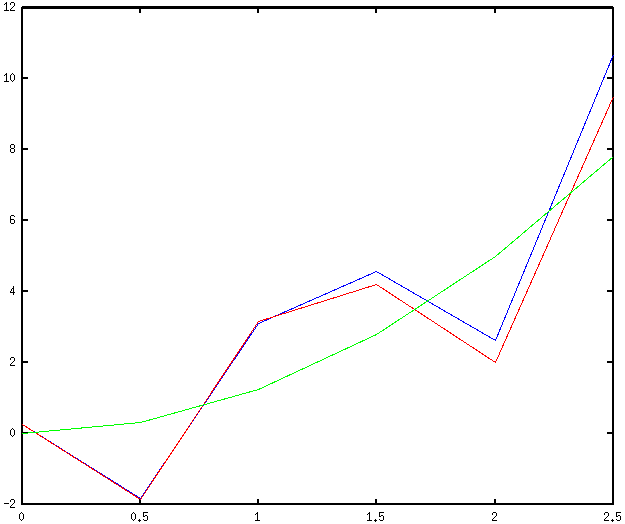
\includegraphics[scale=0.7]{graph}

Rot: GPS Messung, Blau: interpolierte Position, Grün: Reale Position.

\section{Fazit}
Der Kalman-Filter eignet sich durch seine Interpolations- und Echtzeitfähigkeit (durch die Rekursion) sehr gut für derartige Probleme (z.B. Positionsbestimmung). Vor allem der Vergleich der Vorhersage mit der Messung macht ihn sehr effizient.

Die schlechte Qualität des eigenen Ergebnisses lässt auf einen Fehler in dem Modell oder der Implementierung des Algorithmus schliessen, der leider aus Zeitgründen nicht mehr behoben werden kann. Weiterhin ist zu vermuten, dass die Matrix $C$ nicht einfach als $1$ angenommen werden kann.

\end{document}
